\chapter{Hasil dan Pembahasan}


% Berikut ini adalah yang perlu diperhatikan untuk mengisi bab hasil dan pembahasan:

% \begin{enumerate}
% 	\item Setiap rumusan masalah boleh memiliki lebih dari 1 tujuan.
% 	\item Setiap subbab harus spesifik menjawab setiap tujuan yang dituliskan.
% 	\item Setiap rumusan masalah boleh dijawab dengan 1 subbab atau lebih.
% \end{enumerate}

% Berikut ini adalah contoh sub bab untuk menjelaskan tujuan penelitian.

\section{Ringkasan Pelaksanaan Eksperimen}
Bab ini menyajikan dan membahas hasil dari 
metodologi penelitian yang diuraikan di Bab 3. 
Eksperimen dilakukan dengan menjalankan 40 
dataset mahasiswa sintetis  melalui empat 
variasi prompt yang berbeda yaitu:
\begin{itemize}
    \item \textit{Baseline Prompt} : \textit{Prompt} dasar tanpa 
    penambahan konteks apa pun.
    \item Lis Materi : penambahan daftar materi pembelajaran
    yang dipelajari mahasiswa dalam batasan studi kasusnya.
    \item LA : Penambahan analisis \textit{learning analytics}
    berdasarkan data sintetis papan Kanban mahasiswa.
    \item ReAct + LA : Penggabungan metode \textit{Reasoning
    and Acting} (ReAct) dengan analisis \textit{learning analytics}.
\end{itemize}

Eksperimen ini dijalankan pada dua model, 
Llama 3.1 8B Instant dan Llama 3.3 70B Versatile, 
melalui Groq API. 
Hasil respons dari LLM kemudian dievaluasi secara 
kuantitatif (menggunakan BERTScore, BARTScore, dan 
LLM-as-a-Judge)  dan kualitatif 
(melalui penilaian ahli manusia)  untuk menjawab 
tiga pertanyaan penelitian.
% Sub bab pertama adalah membahas tujuan penelitian pertama dengan hasil penelitian ke-1. 
% Dapat ditambahkan beberapa sub bab jika diperlukan.

\section{Analisis Perbandingan Metode Peningkatan Umpan Balik (RQ 1)}
\label{subsection:pembahasan_rq_1}
Pada bagian ini, disajikan hasil eksperimen yang dilakukan
dengan menggunakan empat variasi prompt yang berbeda
untuk menghasilkan umpan balik pedagogis. Hasil dari
umpan balik yang dihasilkan oleh masing-masing variasi prompt
dianalisis menggunakan metrik kuantitatif seperti BERTScore,
BARTScore, dan LLM-as-a-Judge.
Hasil analisis akan dibandingkan untuk menentukan
apakah ada peningkatan umpan balik
dalam konteks pembelajaran daring.

\subsection{Perbandingan Kualitas Semantik}
% Pendahuluan dan tabel ringkasan skor BERTScore dan BARTScore
Pada bagian ini disajikan ringkasan nilai BERTScore 
dan BARTScore yang diperoleh dari 40 dataset untuk 
setiap variasi prompt dan model. Tabel yang akan disajikan 
menampilkan rata-rata keseluruhan untuk masing-masing metrik. 

Berikut adalah tabel hasil evaluasi dengan metode 
BERTScore untuk setiap variasi prompt dan model
yang tertera pada tabel berikut.

% Requires in preamble: \usepackage{tabularx,array}
\begin{table}[H]
\centering
\caption{Ringkasan Hasil BERTScore per Variasi \textit{Context-Engineering}}
\label{tab:BERTScore_summary}
\begin{tabularx}{\textwidth}{l *{3}{>{\centering\arraybackslash}X}|*{3}{>{\centering\arraybackslash}X}}
\hline
Variant & \multicolumn{3}{c}{8B (Llama 3.1 8B)} & \multicolumn{3}{c}{70B (Llama 3.3 70B)} \\ \cline{2-7}
 & {\fontsize{10}{8}\selectfont \textit{Precision}} & {\fontsize{10}{8}\selectfont \textit{Recall}} & {\fontsize{10}{8}\selectfont F1} & {\fontsize{10}{8}\selectfont \textit{Precision}} & {\fontsize{10}{8}\selectfont \textit{Recall}} & {\fontsize{10}{8}\selectfont F1} \\
\hline
\textit{Baseline}        & 0.6505 & 0.6719 & 0.6608 & 0.6567 & 0.6815 & 0.6687 \\
Lis Materi      & 0.6500 & 0.6700 & 0.6597 & 0.6620 & 0.6805 & \textbf{0.6710}  \\
LA              & 0.6586 & 0.6733 & 0.6657 & 0.6529 & 0.6774 & 0.6648  \\
ReAct + LA      & 0.6613 & 0.6716 & \textbf{0.6663} & 0.6561 & 0.6760 & 0.6658  \\
\hline
\end{tabularx}
\end{table}

Dari Tabel \ref{tab:BERTScore_summary}, nilai F1 BERTScore untuk 
model 8B berkisar antara 0,6597 hingga 0,6663, 
dengan variasi prompt "ReAct + LA" memberikan 
nilai tertinggi (0,6663). Sedangkan pada 
model 70B, nilai F1 BERTScore berkisar 
antara 0,6648 hingga 0,6710, di mana variasi 
"Lis Materi" memperoleh skor tertinggi 
(0,6710). Hal ini mengindikasikan bahwa 
untuk model kecil seperti 8B,
penambahan konteks berupa daftar materi 
pembelajaran dan analisis \textit{learning analytics} 
memberikan peningkatan kualitas semantik 
umpan balik yang dihasilkan oleh LLM. 
Namun, untuk model besar seperti 70B,
penambahan konteks yang lebih sederhana
(dalam hal ini hanya daftar materi pembelajaran)
justru memberikan hasil yang lebih baik
dibandingkan dengan penambahan konteks yang
lebih kompleks seperti analisis
\textit{learning analytics} dan metode ReAct.
% \begin{table}[H]
% \centering
% \caption{Ringkasan Precision per variasi prompt (8B vs 70B).}
% \label{tab:precision_scores}
% \begin{tabularx}{\textwidth}{l *{8}{>{\centering\arraybackslash}X}}
% \hline
% Variant & \multicolumn{4}{c}{8B (Llama 3.1 8B)} & \multicolumn{4}{c}{70B (Llama 3.3 70B)} \\ \cline{2-9}
%  & {\fontsize{10}{8}\selectfont Feedback} & {\fontsize{10}{8}\selectfont Motivasi} & {\fontsize{10}{8}\selectfont Apresiasi} & {\fontsize{10}{8}\selectfont \textbf{Overall}} & {\fontsize{10}{8}\selectfont Feedback} & {\fontsize{10}{8}\selectfont Motivasi} & {\fontsize{10}{8}\selectfont Apresiasi} & {\fontsize{10}{8}\selectfont \textbf{Overall}} \\
% \hline
% Baseline        & 0.6349 & 0.6575 & 0.6590 & 0.6505 & 0.6411 & 0.6530 & 0.6759 & 0.6567 \\
% List Materi     & 0.6368 & 0.6564 & 0.6568 & 0.6500 & 0.6487 & 0.6600 & 0.6772 & 0.6620 \\
% LA              & 0.6393 & 0.6675 & 0.6690 & 0.6586 & 0.6416 & 0.6458 & 0.6712 & 0.6529 \\
% LA + ReAct      & 0.6565 & 0.6570 & 0.6705 & 0.6613 & 0.6531 & 0.6451 & 0.6702 & 0.6561 \\
% \hline
% \end{tabularx}
% \end{table}

% \begin{table}[H]
% \centering
% \caption{Ringkasan Recall per variasi prompt (8B vs 70B).}
% \label{tab:recall_scores}
% \begin{tabularx}{\textwidth}{l *{8}{>{\centering\arraybackslash}X}}
% \hline
% Variant & \multicolumn{4}{c}{8B (Llama 3.1 8B)} & \multicolumn{4}{c}{70B (Llama 3.3 70B)} \\ \cline{2-9}
%  & {\fontsize{10}{8}\selectfont Feedback} & {\fontsize{10}{8}\selectfont Motivasi} & {\fontsize{10}{8}\selectfont Apresiasi} & {\fontsize{10}{8}\selectfont \textbf{Overall}} & {\fontsize{10}{8}\selectfont Feedback} & {\fontsize{10}{8}\selectfont Motivasi} & {\fontsize{10}{8}\selectfont Apresiasi} & {\fontsize{10}{8}\selectfont \textbf{Overall}} \\
% \hline
% Baseline        & 0.6753 & 0.6712 & 0.6691 & 0.6719 & 0.6809 & 0.6736 & 0.6900 & 0.6815 \\
% List Materi     & 0.6720 & 0.6680 & 0.6701 & 0.6700 & 0.6775 & 0.6743 & 0.6897 & 0.6805 \\
% LA              & 0.6715 & 0.6692 & 0.6791 & 0.6733 & 0.6747 & 0.6698 & 0.6876 & 0.6774 \\
% LA + ReAct      & 0.6729 & 0.6640 & 0.6780 & 0.6716 & 0.6742 & 0.6666 & 0.6872 & 0.6760 \\
% \hline
% \end{tabularx}
% \end{table}

% Catatan: ganti nilai contoh di atas dengan hasil pengolahan skor aktual Anda.
Selain hasil dari BERTScore, berikut adalah tabel hasil evaluasi dengan metode 
BARTScore untuk setiap variasi prompt dan model
yang tertera pada tabel berikut.

% buat tabel BARTScore di sini
\begin{table}[H]
\centering
\caption{Ringkasan Hasil BARTScore per Variasi \textit{Context-Engineering}}
\label{tab:BARTScore_summary}
\begin{tabularx}{\textwidth}{l *{3}{>{\centering\arraybackslash}X}|*{3}{>{\centering\arraybackslash}X}}
\hline
Variant & \multicolumn{3}{c}{8B (Llama 3.1 8B)} & \multicolumn{3}{c}{70B (Llama 3.3 70B)} \\ \cline{2-7}
 & {\fontsize{9}{10}\selectfont \textit{Precision}} & {\fontsize{9}{10}\selectfont \textit{Recall}} & {\fontsize{9}{10}\selectfont F1-Score} & {\fontsize{9}{10}\selectfont \textit{Precision}} & {\fontsize{9}{10}\selectfont \textit{Recall}} & {\fontsize{9}{10}\selectfont F1-Score} \\
\hline
\textit{Baseline}        & {\fontsize{9}{10}\selectfont -11.0907} & {\fontsize{9}{10}\selectfont -12.3656} & {\fontsize{9}{10}\selectfont -11.7282} & {\fontsize{9}{10}\selectfont -11.1677} & {\fontsize{9}{10}\selectfont -12.2132} & {\fontsize{9}{10}\selectfont -11.6905} \\
Lis Materi      & {\fontsize{9}{10}\selectfont -11.1788} & {\fontsize{9}{10}\selectfont -12.5383} & {\fontsize{9}{10}\selectfont -11.8586} & {\fontsize{9}{10}\selectfont -11.0399} & {\fontsize{9}{10}\selectfont -12.1851} & {\fontsize{9}{10}\selectfont \textbf{-11.6125}} \\
LA              & {\fontsize{9}{10}\selectfont -10.9045} & {\fontsize{9}{10}\selectfont -12.1800} & {\fontsize{9}{10}\selectfont -11.5422} & {\fontsize{9}{10}\selectfont -11.2543} & {\fontsize{9}{10}\selectfont -12.1306} & {\fontsize{9}{10}\selectfont -11.6924} \\
ReAct + LA      & {\fontsize{9}{10}\selectfont -10.5800} & {\fontsize{9}{10}\selectfont -12.2345} & {\fontsize{9}{10}\selectfont \textbf{-11.4073}} & {\fontsize{9}{10}\selectfont -10.8933} & {\fontsize{9}{10}\selectfont -12.4587} & {\fontsize{9}{10}\selectfont -11.6760} \\
\hline
\end{tabularx}
\end{table}

Pada metrik BARTScore (Tabel \ref{tab:BARTScore_summary}), 
semua variasi 
prompt menunjukkan nilai negatif, yang merupakan 
karakteristik dari metrik ini dalam pengukuran 
kualitas teks. Model 8B menunjukkan peningkatan 
performa dari \textit{Baseline} (-11,7282) ke variasi "ReAct + LA" 
(-11,4073), yang berarti kualitas umpan balik secara 
keseluruhan membaik dengan penambahan konteks dan metode 
ReAct. Model 70B juga menunjukkan pola serupa, 
meskipun variasi "Lis Materi" dan "ReAct+ LA" 
memiliki nilai yang cukup berdekatan, dengan "Lis Materi" 
sedikit lebih baik. Untuk model kecil, metrik ini mendukung 
temuan bahwa penambahan konteks dan metode ReAct 
memberikan kontribusi positif terhadap kualitas semantik 
umpan balik. Namun, untuk model besar, semakin diberikan
konteks yang kompleks tidak selalu menghasilkan
peningkatan yang signifikan dalam kualitas semantik.


\subsection{Perbandingan Kualitas Relevansi}
% Pendahuluan dan tabel ringkasan skor LLM-as-a-Judge
Pada bagian ini disajikan ringkasan nilai LLM-as-a-Judge
yang diperoleh dari 40 dataset untuk
setiap variasi prompt dan model. Tabel yang disajikan
menampilkan rata-rata keseluruhan untuk masing-masing metrik.
Berikut adalah tabel hasil evaluasi dengan metode
LLM-as-a-Judge untuk setiap variasi prompt dan model:
% buat tabel LLM-as-a-Judge di sini
\begin{table}[H]
\centering
\caption{Ringkasan Overall LLM-as-a-Judge per Metode}
\label{tab:llm_judge_overall}
\small
\begin{tabularx}{\textwidth}{l *{3}{>{\centering\arraybackslash}X}|*{3}{>{\centering\arraybackslash}X}}
\hline
Metode & \multicolumn{3}{c|}{8B (Llama 3.1 8B)} & \multicolumn{3}{c}{70B (Llama 3.3 70B)} \\ \cline{2-7}
 & \textit{Precision} & \textit{Recall} & F1-Score & \textit{Precision} & \textit{Recall} & F1-Score \\
\hline
\textit{Baseline}        & 1.0000 & 0.4567 & 0.5371 & 1.0000 & 0.6417 & 0.7271 \\
Lis Materi      & 0.9333 & 0.4767 & 0.5627 & 1.0000 & 0.6600 & \textbf{0.7571} \\
LA              & 1.0000 & 0.5017 & 0.5896 & 0.9333 & 0.5717 & 0.6399 \\
ReAct + LA  & 1.0000 & 0.5217 & \textbf{0.6121} & 1.0000 & 0.5883 & 0.6715 \\
\hline
\end{tabularx}
\end{table}

Analisis kualitas relevansi menggunakan metode LLM-as-a-Judge 
memberikan gambaran yang lebih detail terkait aspek relevansi 
umpan balik yang dihasilkan. Dari Tabel \ref{tab:llm_judge_overall}, 
untuk model 8B, variasi "ReAct + LA" memberikan nilai 
F1-Score tertinggi sebesar 0,6121, yang menunjukkan 
keseimbangan terbaik antara presisi dan recall dalam 
menilai relevansi umpan balik. Variasi baseline 
memiliki nilai F1-Score terendah (0,5371), menandakan 
bahwa tanpa konteks tambahan, relevansi umpan balik 
lebih rendah. Pada model 70B, variasi "Lis Materi" 
memberikan nilai F1-Score tertinggi sebesar 0,7571, 
diikuti oleh baseline (0,7271) dan "ReAct + LA" 
(0,6715). Hal ini menunjukkan bahwa pada model yang 
lebih besar, penambahan daftar materi pembelajaran 
secara khusus meningkatkan relevansi umpan balik 
secara signifikan.

\subsection{Analisis Evaluasi Kuantitatif}
Analisis evaluasi kuantitatif pada eksperimen ini 
menunjukkan pola yang konsisten terkait pengaruh variasi 
\textit{prompt} dan ukuran model terhadap kualitas umpan balik 
pedagogis yang dihasilkan. Berdasarkan metrik BERTScore dan 
BARTScore, model 8B (Llama 3.1 8B) menunjukkan peningkatan 
kualitas semantik yang paling signifikan ketika metode 
ReAct dan konteks \textit{learning analytics} (ReAct + LA) 
diterapkan, dengan nilai F1 BERTScore tertinggi sebesar 
0,6663 dan peningkatan BARTScore dari -11,7282 (\textit{Baseline}) 
menjadi -11,4073 (ReAct + LA). Hal ini mengindikasikan 
bahwa penambahan konteks yang kompleks dan metode ReAct 
mampu memperbaiki akurasi dan kualitas semantik umpan 
balik pada model yang lebih kecil.

Sebaliknya, pada model 70B (Llama 3.3 70B), peningkatan 
kualitas semantik lebih optimal dicapai dengan penambahan 
konteks yang lebih sederhana, yakni daftar materi 
pembelajaran (Lis Materi), yang menghasilkan nilai F1 
BERTScore tertinggi sebesar 0,6710 dan BARTScore yang 
lebih baik dibandingkan variasi lain. Penambahan
konteks kompleks seperti LA dan ReAct + LA tidak 
memberikan peningkatan signifikan, bahkan cenderung 
stagnan atau sedikit menurun. Ini menunjukkan bahwa 
model besar mungkin sudah memiliki kapasitas internal 
yang cukup untuk memahami konteks pembelajaran, sehingga 
konteks tambahan yang terlalu kompleks tidak selalu 
memperbaiki hasil.

Dari sisi relevansi umpan balik yang diukur menggunakan 
metode \textit{LLM-as-a-Judge}, model 8B kembali menunjukkan 
performa terbaik dengan variasi ReAct + LA, yang 
menghasilkan F1-Score tertinggi 0,6121. Ini menegaskan 
bahwa ReAct dan analisis \textit{learning analytics} 
memberikan kontribusi positif dalam meningkatkan relevansi 
umpan balik pada model berukuran kecil. Sedangkan pada 
model 70B, variasi Lis Materi mendominasi dengan F1-Score 
0,7571, menandakan bahwa penambahan konteks berupa daftar 
materi pembelajaran secara khusus meningkatkan relevansi 
umpan balik secara signifikan, lebih baik dibandingkan 
Baseline dan ReAct + LA.

Secara keseluruhan, evaluasi kuantitatif ini mengindikasikan 
bahwa strategi peningkatan umpan balik pedagogis perlu 
disesuaikan dengan kapasitas model LLM yang digunakan. 
Model kecil memperoleh manfaat lebih besar dari penambahan 
konteks yang kompleks dan metode ReAct, sedangkan 
model besar lebih efektif dengan konteks yang sederhana 
dan fokus pada materi pembelajaran. Pendekatan ini 
penting untuk mengoptimalkan kualitas semantik dan 
relevansi umpan balik dalam aplikasi pembelajaran daring.

Dari hasil evaluasi kuantitatif menggunakan 
BERTScore, BARTScore, dan \textit{LLM-as-a-Judge}, diputuskan untuk
mengambil Llama 3.1 8B dengan variasi "ReAct + LA" 
untuk di analisis kualitatif lebih lanjut pada bagian berikutnya.
Hal ini karena pada eksperimen kuantitatif, model memberikan
hasil pengamatan eksperimen yang sejalan dengan seiring 
bertambahnya konteks yang diberikan, semakin baik hasilnya.
Alasan untuk tidak diambilnya Llama 3.3 70B adalah karena pada
model tersebut, semakin banyak konteks yang diberikan, hasil 
yang didapatkan semakin menurun sehingga perlu diketahui terlebih
dahulu penyebabnya terjadinya hal tersebut. Pemilihan model yang
lebih kecil juga mendukung efisiensi komputasi dan kecepatan 
respons sehingga lebih praktis untuk diterapkan dalam skala luas.
Dengan begitu, analisis kualitatif dapat difokuskan pada model yang
menunjukkan potensi terbaik dalam efisiensinya.

% Dari hasil BERTScore, terlihat bahwa model 8B 
% memperoleh peningkatan kualitas semantik umpan 
% balik tertinggi pada variasi "ReAct + LA" dengan 
% nilai F1 sebesar 0,6663. Hal ini menunjukkan bahwa 
% penggabungan metode reasoning dan analisis learning 
% analytics secara sinergis memperbaiki akurasi dan 
% keutuhan konteks semantik dalam umpan balik 
% yang dihasilkan oleh model kecil. Sebaliknya, 
% pada model 70B, variasi "Lis Materi" memberikan 
% hasil terbaik dengan F1 sebesar 0,6710, menandakan 
% bahwa penambahan konteks berupa daftar materi p
% embelajaran sudah cukup untuk meningkatkan kualitas 
% semantik pada model yang lebih besar, tanpa perlu 
% tambahan kompleksitas seperti reasoning atau analisis 
% learning analytics.

% Hasil BARTScore mendukung temuan tersebut dengan pola 
% yang serupa, di mana model 8B menunjukkan peningkatan 
% performa dari baseline ke "ReAct + LA", mengindikasikan 
% bahwa konteks dan metode reasoning berkontribusi positif 
% terhadap kualitas teks. Namun, model 70B menunjukkan 
% perbedaan yang lebih kecil antar variasi, dengan "Lis Materi" 
% sedikit unggul, yang mengindikasikan bahwa kompleksitas 
% konteks tambahan tidak selalu berbanding lurus dengan 
% peningkatan kualitas pada model besar.

% Evaluasi menggunakan LLM-as-a-Judge yang mengukur 
% relevansi umpan balik juga memperlihatkan pola konsisten. 
% Pada model 8B, variasi "ReAct + LA" menghasilkan nilai 
% MacroF1 tertinggi (0,6121), menunjukkan keseimbangan 
% terbaik antara presisi dan recall dalam relevansi umpan 
% balik. Sementara itu, model 70B menunjukkan nilai 
% tertinggi pada variasi "Lis Materi" (MacroF1 0,7571), 
% mengindikasikan bahwa penambahan konteks sederhana 
% berupa daftar materi pembelajaran cukup efektif untuk 
% meningkatkan relevansi umpan balik pada model yang 
% lebih besar.

% Secara keseluruhan, analisis kuantitatif ini menggarisbawahi 
% bahwa peningkatan kualitas umpan balik tidak hanya bergantung 
% pada kompleksitas konteks yang diberikan, tetapi juga sangat 
% dipengaruhi oleh kapasitas model yang digunakan. Model kecil 
% (8B) mendapatkan manfaat yang lebih signifikan dari kombinasi 
% konteks dan metode reasoning yang kompleks, sedangkan model 
% besar (70B) cenderung merespon lebih baik terhadap konteks 
% yang sederhana dan fokus. Temuan ini memberikan arahan penting 
% dalam perancangan prompt context-engineering yang efisien dan 
% efektif sesuai dengan kapasitas model LLM yang digunakan.

% Secara keseluruhan, hasil analisis pada kedua 
% metrik tersebut mengindikasikan bahwa penambahan 
% konteks pembelajaran dan integrasi metode \textit{reasoning} 
% seperti ReAct dengan \textit{learning analytics} dapat 
% meningkatkan kualitas semantik dan relevansi umpan 
% balik pedagogis yang dihasilkan oleh \textit{LLM}. Namun, 
% peningkatan ini bervariasi tergantung pada model 
% yang digunakan dan jenis konteks yang ditambahkan. 
% Model besar seperti 70B cenderung memberikan hasil yang lebih baik 
% secara keseluruhan, terutama dalam aspek relevansi, 
% sementara model 8B menunjukkan peningkatan yang lebih 
% nyata ketika metode ReAct digabungkan dengan 
% \textit{learning analytics}. Temuan ini mendukung hipotesis 
% bahwa pengayaan konteks dan metode \textit{reasoning} dapat 
% memperbaiki kualitas umpan balik dalam pembelajaran 
% daring, meskipun perlu diperhatikan bahwa peningkatan 
% kualitas tidak selalu linier dan bergantung pada 
% kombinasi metode dan model yang digunakan.

\section{Analisis Pengaruh Ukuran Model (RQ 3)}
Pada bagian ini, dilakukan analisis untuk menjawab 
\textit{research question} ketiga (RQ 3) mengenai 
pengaruh ukuran model \textit{Large Language Model} 
(LLM) terhadap kualitas umpan balik pedagogis. 
Analisis ini membandingkan performa antara model Llama 
3.1 8B (model kecil) dan Llama 3.3 70B (model besar) 
menggunakan data kuantitatif yang telah disajikan pada
Subbab \ref{subsection:pembahasan_rq_1}.

\subsection{Perbandingan Kapasitas Dasar (Baseline Performance)} 
Untuk memahami pengaruh ukuran model, langkah pertama adalah 
membandingkan performa dasar (\textit{Baseline}) kedua model, 
yaitu ketika tidak ada \textit{context-engineering} tambahan 
yang diterapkan.

\begin{table}[H]
\centering
\caption{Perbandingan Kinerja \textit{Baseline} Antara Model 8B dan 70B}
\label{tab:baseline_comparison}
\begin{tabularx}{\textwidth}{l >{\centering\arraybackslash}X >{\centering\arraybackslash}X c}
    \hline
    Metrik (F1-Score) & 8B (Llama 3.1 8B) & 70B (Llama 3.3 70B) & Pemenang \\
    \hline
    BERTScore       & 0.6608   & 0.6687   & \textbf{70B} \\
    BARTScore       & -11.7282 & -11.6905 & \textbf{70B} \\
    LLM-as-a-Judge  & 0.5371   & 0.7271   & \textbf{70B} \\
    \hline
\end{tabularx}
\end{table}

Tabel \ref{tab:baseline_comparison} menunjukkan tren yang 
sangat jelas. Model 70B secara konsisten mengungguli model 
8B di semua metrik evaluasi pada kondisi \textit{Baseline}. 
Keunggulan paling signifikan terlihat pada metrik 
\textit{LLM-as-a-Judge}, di mana model 70B (0,7271) 
menunjukkan skor relevansi yang jauh lebih tinggi 
dibandingkan model 8B (0,5371). Pada metrik semantik 
(BERTScore dan BARTScore), model 70B juga menunjukkan 
skor yang sedikit lebih baik. Hal ini mengindikasikan 
bahwa model yang lebih besar (70B) memiliki kapasitas 
internal yang lebih superior dalam menghasilkan umpan 
balik yang relevan dan koheren secara semantik, bahkan 
tanpa konteks tambahan.

\subsection{Analisis Responsivitas terhadap \textit{Context-Engineering}} 
Tren yang lebih kompleks muncul ketika 
menganalisis bagaimana kedua model merespons 
penambahan konteks (\textit{context-engineering}). 
Gambar \ref{fig:pgfplots_bars} membandingkan skor \textit{Baseline} 
dengan skor terbaik yang dicapai oleh variasi 
\textit{prompt} untuk masing-masing model.

\begin{figure}[H]
  \centering
  % --- BERTScore (positif: label di atas batang) ---
  \begin{subfigure}{0.9\textwidth}
    \centering
    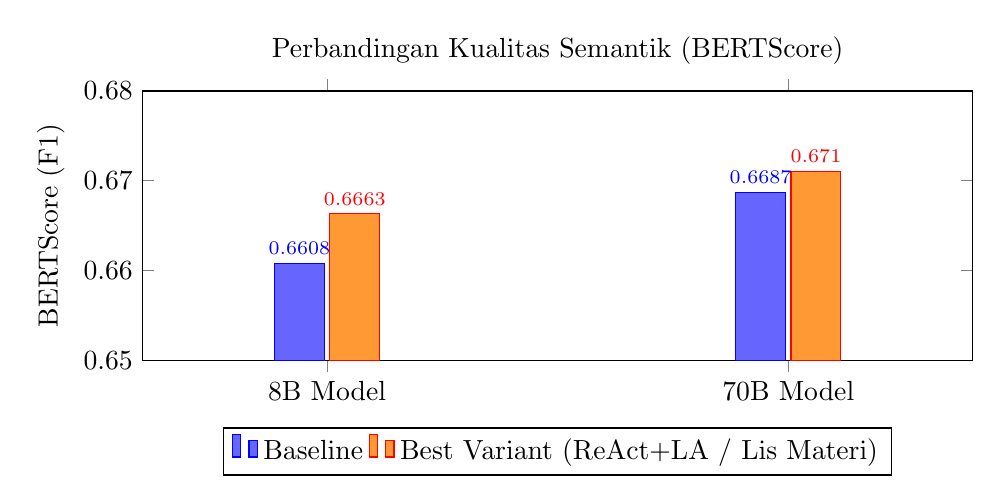
\begin{tikzpicture}
      \begin{axis}[
        ybar,
        bar width=18pt,
        width=\textwidth,
        height=5cm,
        symbolic x coords={8B Model,70B Model},
        xtick=data,
        ymin=0.65,ymax=0.68,
        ylabel={BERTScore (F1)},
        title={Perbandingan Kualitas Semantik (BERTScore)},
        nodes near coords,
        every node near coord/.append style={
          font=\scriptsize,
          anchor=south,   % label di atas batang
          yshift=2pt,     % geser sedikit ke atas
          inner sep=1pt
        },
        nodes near coords style={
          /pgf/number format/fixed,
          /pgf/number format/precision=4
        },
        enlarge x limits=0.4,
        legend style={at={(0.5,-0.25)},anchor=north,legend columns=2}
      ]
        \addplot+[fill=blue!60] coordinates {(8B Model,0.6608) (70B Model,0.6687)};
        \addplot+[fill=orange!80] coordinates {(8B Model,0.6663) (70B Model,0.6710)};
        \legend{Baseline, Best Variant (ReAct+LA / Lis Materi)}
      \end{axis}
    \end{tikzpicture}
  \end{subfigure}

  \vspace{6pt}

  % --- BARTScore (negatif: gunakan anchor=north dan yshift negatif) ---
  \begin{subfigure}{0.9\textwidth}
    \centering
    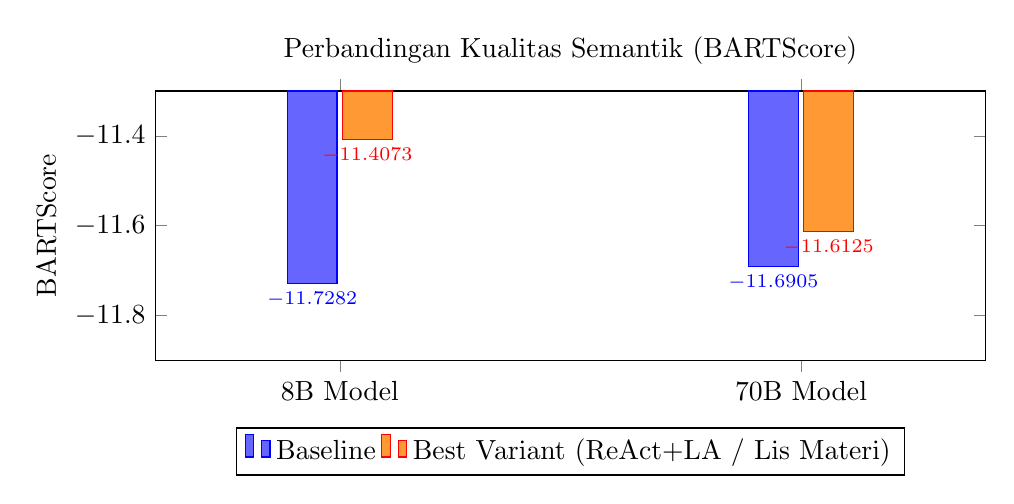
\begin{tikzpicture}
      \begin{axis}[
        ybar,
        bar width=18pt,
        width=\textwidth,
        height=5cm,
        symbolic x coords={8B Model,70B Model},
        xtick=data,
        ymin=-11.9,ymax=-11.3,
        ylabel={BARTScore},
        title={Perbandingan Kualitas Semantik (BARTScore)},
        nodes near coords,
        every node near coord/.append style={
          font=\scriptsize,
          anchor=north,  % untuk batang negatif, anchor ke utara (agar label "di atas" batang)
          yshift=-2pt,   % geser sedikit ke atas relatif ke batang negatif
          inner sep=1pt
        },
        nodes near coords style={
          /pgf/number format/fixed,
          /pgf/number format/precision=4
        },
        enlarge x limits=0.4,
        legend style={at={(0.5,-0.25)},anchor=north,legend columns=2}
      ]
        \addplot+[fill=blue!60] coordinates {(8B Model,-11.7282) (70B Model,-11.6905)};
        \addplot+[fill=orange!80] coordinates {(8B Model,-11.4073) (70B Model,-11.6125)};
        \legend{Baseline, Best Variant (ReAct+LA / Lis Materi)}
      \end{axis}
    \end{tikzpicture}
  \end{subfigure}

  \vspace{6pt}

  % --- LLM-as-a-Judge (positif: label di atas batang) ---
  \begin{subfigure}{0.9\textwidth}
    \centering
    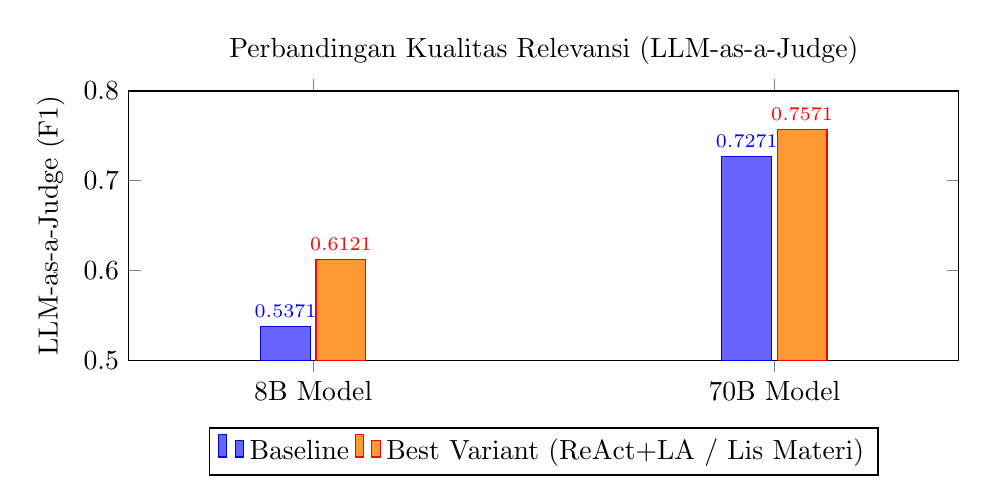
\begin{tikzpicture}
      \begin{axis}[
        ybar,
        bar width=18pt,
        width=\textwidth,
        height=5cm,
        symbolic x coords={8B Model,70B Model},
        xtick=data,
        ymin=0.5,ymax=0.8,
        ylabel={LLM-as-a-Judge (F1)},
        title={Perbandingan Kualitas Relevansi (LLM-as-a-Judge)},
        nodes near coords,
        every node near coord/.append style={
          font=\scriptsize,
          anchor=south,   % label di atas batang
          yshift=2pt,     % geser sedikit ke atas
          inner sep=1pt
        },
        nodes near coords style={
          /pgf/number format/fixed,
          /pgf/number format/precision=4
        },
        enlarge x limits=0.4,
        legend style={at={(0.5,-0.25)},anchor=north,legend columns=2}
      ]
        \addplot+[fill=blue!60] coordinates {(8B Model,0.5371) (70B Model,0.7271)};
        \addplot+[fill=orange!80] coordinates {(8B Model,0.6121) (70B Model,0.7571)};
        \legend{Baseline, Best Variant (ReAct+LA / Lis Materi)}
      \end{axis}
    \end{tikzpicture}
  \end{subfigure}

  \caption{Perbandingan Kinerja Model 8B vs 70B pada metrik evaluasi berbeda.}
  \label{fig:pgfplots_bars}
\end{figure}

Perbandingan kinerja antara model 8B dan 70B 
pada ketiga metrik evaluasi (BERTScore, 
BARTScore, dan \textit{LLM-as-a-Judge}) dapat dilihat 
pada gambar berikut. Gambar \ref{fig:pgfplots_bars} 
ini membandingkan 
skor F1 dari variasi \textit{Baseline} dengan 
skor F1 dari variasi \textit{prompt} terbaik 
untuk setiap model.

Pada metrik BERTScore, model 70B \textit{Baseline} 
(0.6687) sudah lebih tinggi daripada skor terbaik 
model 8B (0.6663). Model 70B hanya mengalami sedikit 
peningkatan ke 0.6710 dengan \textit{Lis Materi}. 
Sebaliknya, model 8B menunjukkan peningkatan yang 
lebih besar dari \textit{Baseline} (0.6608) ke \textit{ReAct + LA} 
(0.6663).

Pada metrik BARTScore, model 8B menunjukkan peningkatan 
paling substansial, bergerak dari -11.7282 
(\textit{Baseline}) ke -11.4073 (\textit{ReAct + LA}), 
sebuah peningkatan yang signifikan. Model 70B juga 
meningkat, namun dengan margin yang lebih kecil, dari 
-11.6905 (\textit{Baseline}) ke -11.6125 (\textit{Lis Materi}).

Pada metrik \textit{LLM-as-a-Judge}, kedua model menunjukkan 
peningkatan. Model 8B meningkat dari 0.5371 
(\textit{Baseline}) ke 0.6121 (\textit{ReAct + LA}). 
Model 70B, meskipun sudah memiliki \textit{Baseline} 
yang sangat tinggi (0.7271), masih dapat meningkat ke 
0.7571 dengan \textit{Lis Materi}.

Temuan kuantitatif ini, khususnya perbedaan performa 
yang signifikan pada metrik \textit{LLM-as-a-Judge}, 
dapat dijelaskan lebih lanjut melalui analisis 
kualitatif terhadap luaran aktual dari kedua 
model dibandingkan dengan \textit{ground truth}. 
Analisis kualitatif menunjukkan bahwa Llama 70B 
secara jelas lebih unggul daripada Llama 8B. Alasan 
utamanya adalah Llama 70B lebih berhasil menangkap 
\textit{niat pedagogis} dari \textit{ground truth}, 
sementara Llama 8B cenderung gagal dalam eksekusi dan 
hanya melaporkan data secara harfiah.
Perbedaan mendalam ini dapat diuraikan menjadi tiga poin utama:

\begin{enumerate} 
    \item \textbf{Kualitas Feedback: Preskriptif (70B) vs. Deskriptif (8B)}
    Perbedaan paling signifikan terletak pada \textit{apa}
yang dilakukan oleh \textit{feedback} tersebut.
\begin{itemize}
    \item \textbf{\textit{Ground truth}:} \textit{Feedback} bersifat
    preskriptif dan metakognitif. Ia tidak hanya melaporkan
    masalah, tetapi memberikan strategi belajar yang konkret
    dan dapat ditindaklanjuti.
    \begin{quote}
    Contoh: "Fokus menuntaskan satu kartu sampai 'Done'...",
    "Hindari pindah kolom sebelum item inti selesai."
    \end{quote}
    
    \item \textbf{Llama 3.3 70B (Baik):} Model ini \textit{mencoba}
    menjadi preskriptif. Ia menganalisis data dan memberikan
    saran langkah berikutnya yang spesifik.
    \begin{quote}
    Contoh: "Pertimbangkan untuk menyelesaikan checklist
    yang tersisa...", "Untuk memperbaiki ini, Anda perlu
    memfokuskan diri pada..."
    \end{quote}
    
    \item \textbf{Llama 3.1 8B (Kurang):} Model ini hampir
    seluruhnya bersifat deskriptif. Ia hanya melaporkan
    data yang dilihatnya dan kemudian mengajukan
    pertanyaan generik, tanpa memberikan solusi atau strategi.
    \begin{quote}
    Contoh: "Saya melihat bahwa Anda memiliki satu kartu
    di Planning...", "Saya ingin tahu apa yang menyebabkan
    Anda terhambat..."
    \end{quote}
\end{itemize}
Kesimpulannya, Llama 3.3 70B bertindak sebagai pembimbing
(sesuai \textit{ground truth}), sedangkan Llama 3.1 8B
hanya bertindak sebagai pelapor data.

\item \textbf{Pemisahan Fungsi: Apresiasi (70B) vs. Kritik (8B)}

Terdapat kegagalan pada Llama 3.1 8B yang berhasil
diatasi oleh Llama 3.3 70B, yang juga sejalan dengan kritik
ahli pada Subbab \ref{subsection:analisis_kualitatif_terbuka}.
\begin{itemize}
    \item \textbf{\textit{Ground truth} (Target):} Apresiasinya
    bernilai murni, singkat, dan positif. Tujuannya hanya
    untuk validasi emosional.
    \begin{quote}
    Contoh: "Good job, tinggal dipertahankan.",
    "Keberanian memulai adalah langkah penting."
    \end{quote}
    
    \item \textbf{Llama 3.3 70B (Baik):} Model ini berhasil
    menjaga apresiasi tetap murni. Responnya fokus pada
    validasi usaha dan tidak mencampurnya dengan kritik.
    \begin{quote}
    Contoh: "Anda telah mengambil langkah awal yang baik...",
    "Ini adalah langkah yang sangat baik dan patut diapresiasi."
    \end{quote}
    
    \item \textbf{Llama 3.1 8B (Gagal):} Sementara model ini mengalami
    "kontaminasi respon". Ia tidak bisa memberikan apresiasi
    murni dan hampir selalu mencampurnya dengan \textit{feedback}
    korektif, yang ditandai dengan kata "tetapi".
    \begin{quote}
    Contoh: "Saya mengapresiasi usaha Anda..., \textbf{tetapi}
    saya ingin Anda terus maju...", "Saya mengapresiasi
    usaha Anda..., \textbf{tetapi} masih ada banyak
    yang belum diselesaikan."
    \end{quote}
\end{itemize}
Kesimpulannya, Llama 70B memahami bahwa \textit{apresiasi}
memiliki fungsi afektif yang terpisah, sementara Llama 8B
gagal membedakan fungsi ini.

\item \textbf{Variasi Linguistik dan Kepatuhan Persona}

Ukuran model yang lebih besar secara langsung
berdampak pada kekayaan linguistik.
\begin{itemize}
    \item \textbf{\textit{Ground truth} :} Memiliki variasi
    yang tinggi. Kata-kata motivasinya beragam: "Bangun
    momentum...", "Jaga ritme...", "Tetapkan target kecil...".
    
    \item \textbf{Llama 3.3 70B (Baik):} Menunjukkan variasi
    yang jauh lebih baik. Respon \textit{motivasi}-nya
    lebih kontekstual dan tidak terlalu formulaik.
    \begin{quote}
    Contoh: "Sekarang, cobalah untuk meningkatkan
    kompetensi Anda...", "Apa yang Anda pikirkan tentang
    memulai dengan menyelesaikan satu checklist lagi...?"
    \end{quote}
    
    \item \textbf{Llama 3.1 8B (Kurang):} Sangat monoton dan
    repetitif. Model ini terjebak pada beberapa frasa
    formulaik, terutama pada \textit{motivasi}.
    \begin{quote}
    Contoh: "Saya percaya bahwa Anda memiliki kemampuan
    untuk..." dan "Anda memiliki kemampuan untuk..."
    diulang di hampir setiap respon (temuan ini juga
    dikonfirmasi oleh ahli pada 4.4.2).
    \end{quote}
\end{itemize}
Kesimpulannya, ukuran model 70B yang lebih besar
memungkinkannya memiliki variasi linguistik yang
lebih kaya, membuatnya terdengar lebih natural
dan tidak robotik.
\end{enumerate}

\subsection{Interpretasi Tren dan Analisis} 
Setelah dilakukannya analisis komparatif antara model 8B dan 70B,
dapat disimpulkan beberapa hal terkait pengaruh ukuran model
terhadap kualitas umpan balik pedagogis yang dihasilkan.
% Analisis komparatif ini menghasilkan dua temuan utama:

\begin{enumerate} 
    \item \textbf{Kapasitas Dasar Unggul pada Model Besar}: 
    Model 70B memiliki kapasitas dasar yang jauh lebih tinggi, 
    terutama dalam hal relevansi (\textit{LLM-as-a-Judge}). 
    Skor \textit{Baseline}-nya bahkan melampaui skor 
    terbaik yang bisa dicapai model 8B dengan konteks 
    paling kompleks sekalipun. 
    \item \textbf{Responsivitas Konteks Berbeda}: Model 
    8B (kecil) menunjukkan \textbf{responsivitas yang lebih tinggi} 
    terhadap \textit{context-engineering} yang kompleks pada 
    pengukuran BERTScore, BARTScore, dan \textit{LLM-as-a-Judge}. 
    Peningkatan performa terbesar pada model 8B terjadi 
    pada variasi "ReAct + LA", seperti yang terlihat jelas 
    pada peningkatan skor BARTScore. Hal ini mengindikasikan 
    bahwa model kecil sangat bergantung pada \textit{prompt} 
    yang terstruktur dan kaya konteks untuk mengkompensasi 
    keterbatasan kapasitas internalnya. Hal ini juga didukung
    oleh literatur \cite{Tang2025FewShot, pawlik2025choice} yang 
    menyatakan bahwa model
    kecil cenderung lebih sensitif terhadap jumlah teknik 
    \textit{prompt engineering} yang digunakan dibandingkan model besar.

    \item \textbf{Efisiensi Konteks pada Model Besar}: 
    Sebaliknya, LLM 70B (besar) \textbf{tidak terlalu diuntungkan} 
    oleh konteks yang kompleks. Performa terbaiknya justru dicapai 
    dengan konteks yang lebih sederhana ("Lis Materi"). Penambahan 
    konteks "ReAct + LA" yang kompleks bahkan cenderung menurunkan 
    performanya (misalnya pada BERTScore dan \textit{LLM-as-a-Judge}) 
    dibandingkan dengan "Lis Materi". Hal ini juga didukung oleh literatur
    \cite{Tang2025FewShot, pawlik2025choice} di mana model 
    besar cenderung kurang sensitif 
    terhadap penambahan jumlah teknik \textit{prompt engineering} yang
    digunakan dibandingkan model kecil. Namun, perlu dicatat,
    pada literatur \cite{Tang2025FewShot}, model dengan ukuran 70B
    tidak disebutkan secara eksplisit, sehingga perlu penelitian lebih lanjut
    untuk mengonfirmasi temuan ini pada model Llama 3.3 70B.
    Terdapat dugaan bahwa dalam eksperimen penelitian ini, ketika
    \textit{context-engineering} menjadi terlalu kompleks membuat
    model besar performanya "dipaksa" meniru luaran dari model Llama 3.1 8B,
    alih-alih mendekati \textit{ground truth}. Terbukti dengan
    contoh luaran yang dihasilkan pada variasi "ReAct + LA" oleh
    Llama 3.3 70B yang cenderung meniru gaya bahasa
    Llama 3.1 8B yang deskriptif dan kurang preskriptif.
    Contoh luaran ini adalah seperti ini.
    \begin{itemize}
        \item \textbf{Llama 3.3 70B (ReAct + LA):}
        \begin{quote}
            "Anda memiliki 1 kartu di fase Planning...", 
            "rasio selesai masih 0\%. Perlu diperhatikan juga bahwa ada alert REFLECTION\_DEBT...", 
            "Ini menunjukkan bahwa proses belajar Anda sedang terhambat."
        \end{quote}
        \item \textbf{Llama 3.1 8B (ReAct + LA):}
        \begin{quote}
            "Saya melihat bahwa Anda 
            memiliki satu kartu di Planning...", 
            "Checklist selesai hanya 33,33\%...", 
            "Saya ingin tahu apa yang menyebabkan Anda terhambat..."
        \end{quote}
    \end{itemize}
    Luaran Llama 3.3 70B di atas menunjukkan gaya bahasa
    yang sangat mirip dengan Llama 3.1 8B,
    yang bersifat deskriptif dan kurang memberikan
    solusi konkret, berbeda dengan \textit{ground truth} yang
    bersifat preskriptif. Hal ini mengindikasikan bahwa adanya
    kemungkinan penambahan konteks yang 
    terlalu kompleks pada model besar
    justru memaksa model untuk meniru gaya bahasa
    model kecil, sehingga menurunkan kualitas umpan balik
    yang dihasilkannya.
    
\end{enumerate}

Kesimpulannya, pengaruh ukuran model bersifat dua arah. 
Model besar (70B) memberikan kualitas dasar yang lebih 
baik, namun model kecil (8B) memperoleh manfaat yang jauh 
lebih besar dari strategi \textit{context-engineering} yang 
canggih. Hal ini juga menjelaskan keputusan yang diambil 
pada RQ 1 di mana model 70B tidak dianalisis lebih lanjut karena 
penambahan konteks kompleks justru menurunkan kinerjanya, 
sehingga hasil tersebut yang perlu diinvestigasi 
terpisah dipenelitian berikutnya. Sebaliknya, 
model 8B dengan "ReAct + LA" dipilih karena menunjukkan pola 
yang logis (peningkatan performa sejalan dengan penambahan 
konteks) dan menawarkan efisiensi komputasi yang lebih 
praktis.

% Tapi kenapa untuk model yang 8B semakin diberikan tugas teknik context engineering yang kompleks, semakin bagus nilai BERTScore dan BARTScore nya? Tidak seperti 70B yang berkebalikan


% The differences in how 8B and 70B large language models (LLMs) respond to complex context engineering can be attributed to several factors:

% Capacity and Efficiency: The 70B model has a larger parameter size, enabling it to naturally capture more intricate patterns and nuances in the language without relying heavily on complex prompts. Conversely, the 8B model, being smaller, might benefit more from detailed prompts, which can provide additional cues and context it might not capture on its own.

% Focus and Disambiguation: For a smaller model like the 8B, complex prompts can help disambiguate instructions and focus the model's attention on the specific task, potentially boosting its performance. Meanwhile, the 70B model might already excel at handling diverse linguistic structures, making complex prompts less necessary and sometimes even counterproductive if they introduce noise or irrelevant complexity.

% Prompt Engineering Benefits: Smaller models often gain more from prompt engineering because it can serve as a guide or scaffold, assisting these models in focusing on specific details that they might not inherently prioritize. In contrast, larger models typically have more inherent capacity and don't need as much external guidance through tailored prompts.

% Data Dependency and Specialization: The performance improvements in the 8B model with complex prompts might also be a result of how its training data aligns with the prompt strategy used. Models can have optimizations and learnings that align better with certain styles of prompts, leading to benefits when such prompts are used.

% Differential Performance across Models: As larger models often require substantial resources and finely tuned prompts may not make as significant a difference in outcome because slight improvements are already achieved through their sheer size, smaller models can exhibit more visible gains when complex prompts are correctly applied, as these guide their more limited capacity toward optimal performance.

% Thus, while both models may derive some benefit from engineered prompts, the additional complexity can be more salient and beneficial for the 8B model as a support mechanism for its smaller capacity, enhancing its BERTScore and BARTScore significantly compared to the 70B model, which naturally excels with simpler prompts due to its larger inherent capabilities.

\section{Validasi dan Persepsi Ahli Manusia (RQ 2)}
Untuk menjawab \textit{research question} kedua (\textit{RQ 2}) mengenai 
persepsi ahli manusia terhadap kualitas respon yang 
dihasilkan oleh \textit{Feedback Agent}, dilakukan proses validasi pakar. 
Validasi ini bertujuan untuk menilai efektivitas \textit{Feedback Agent} 
sebagai asisten pembelajaran dalam memberikan \textit{feedback}, 
\textit{motivation}, dan \textit{appreciation}. Proses ini melibatkan seorang ahli 
dalam bidang Psikologi Pembelajaran, Shafira Anissa, dari 
Universitas Gadjah Mada.

Penilaian pakar dilakukan menggunakan instrumen kuesioner 
terstruktur yang mencakup tiga aspek utama: \textit{Feedback Quality} 
(Kualitas Umpan Balik), \textit{Motivational Support} 
(Dukungan Motivasi), dan \textit{Appreciation/Affective Support} 
(Apresiasi dan Penguatan Emosional). 
Pakar memberikan penilaian kuantitatif menggunakan skala \textit{Likert} 1--5  
serta umpan balik kualitatif melalui pertanyaan terbuka.
\subsection{Analisis Penilaian Rubrik Ahli Manusia}
Penilaian kuantitatif oleh pakar dirangkum berdasarkan 15 
butir pertanyaan yang mewakili tiga aspek evaluasi. Skor 1 
mewakili "Sangat Tidak Setuju", 2 "Tidak Setuju", 3 "Netral", 4 
"Setuju", dan 5 "Sangat Setuju".


\subsubsection{Aspek Kualitas Umpan Balik} 
Aspek ini menilai seberapa informatif, 
jelas, relevan, dan konstruktif 
umpan balik yang diberikan chatbot. Hasil penilaian pakar 
adalah sebagai berikut dapat dilihat pada Tabel \ref{tab:expert_feedback_quality}:

\begin{table}[H]
\centering
\caption{Penilaian Aspek \textit{Feedback} Umpan Balik oleh Pakar}
\label{tab:expert_feedback_quality}
\begin{tabularx}{\textwidth}{l X >{\centering\arraybackslash}p{1.2cm}}
\hline
Indikator & Pertanyaan Angket & Skor \\
\hline
F1 (Kejelasan) & Feedback dari chatbot mudah saya pahami. & 4 \\
F2 (Spesifisitas) & Chatbot memberikan saran perbaikan yang spesifik terhadap pekerjaan saya. & 4 \\
F3 (Relevansi) & Feedback dari chatbot sesuai dengan aktivitas belajar yang sedang saya lakukan. & 3 \\
F4 (Konstruktivitas) & Umpan balik dari chatbot membantu saya memperbaiki kesalahan dalam belajar. & 4 \\
F5 (Feed-forward) & Chatbot memberikan arahan atau langkah selanjutnya yang dapat saya lakukan. & 4 \\
\hline
\end{tabularx}
\end{table}


% F1 (Kejelasan): 4 (Setuju)

% F2 (Spesifisitas): 4 (Setuju)

% F3 (Relevansi): 3 (Netral)

% F4 (Konstruktivitas): 4 (Setuju)

% F5 (Feed-forward): 4 (Setuju)

% Mayoritas indikator feedback dinilai positif ("Setuju"). 
% Namun, indikator Relevansi (F3) mendapat nilai "Netral", 
% yang mengindikasikan bahwa kesesuaian umpan balik dengan 
% aktivitas pengguna terkadang belum optimal.

Aspek ini secara umum dinilai positif (Skor 4, "Setuju") 
pada mayoritas indikator, seperti Kejelasan (F1), Spesifisitas 
(F2), Konstruktivitas (F4), dan Feed-forward (F5). Hal ini 
menunjukkan \textit{chatbot} telah berhasil menyampaikan umpan balik 
yang dapat dipahami dan berorientasi pada perbaikan. Namun, 
skor Netral (Skor 3) pada F3 (Relevansi) menjadi catatan kritis. 
Ini mengindikasikan bahwa meskipun umpan balik yang diberikan 
berkualitas baik, namun terkadang belum sepenuhnya relevan 
atau selaras dengan konteks aktivitas spesifik yang sedang 
dilakukan pengguna.

Kekurangan ini terletak pada kurangnya spesifisitas kontekstual. 
Sebagai contoh, respon seperti "Saya melihat bahwa Anda memiliki 
satu kartu di Planning..." atau "kartu yang masih dalam fase Monitoring..." 
tidak secara eksplisit menyebutkan \textit{nama} kartu yang dimaksud. Hal 
ini membuat umpan balik terasa generik dan kurang relevan, terutama 
jika pengguna memiliki beberapa kartu dalam fase yang sama. Sebaliknya, 
respon yang lebih efektif 
% (seperti pada data contoh 10) 
secara 
spesifik menyebutkan nama kartu, seperti 
"'Object Oriented Programming [CS101]'". Inkonsistensi dalam menyebutkan 
konteks spesifik inilah yang diduga kuat menjadi penyebab skor F3 
(Relevansi) dinilai Netral.

Analisis tersebut didukung dengan hasil wawancara
dengan ahli. Ahli secara eksplisit mengkritik bahwa feedback 
"nggak spesifik"  pada \textit{timestamp} [00:02:23,946]. Contohnya adalah \textit{chatbot} mengatakan 
"kamu ada lho kartu yang masih di fase planning... tapi kartu yang mana?" 
(\textit{timestamp} [00:02:23,946]).

\subsubsection{Aspek Dukungan Motivasi} 
Berikutnya, aspek ini menilai kemampuan chatbot dalam meningkatkan motivasi 
belajar. Hasil penilaian pakar dapat dilihat pada Tabel \ref{tab:expert_motivational_support}:
\begin{table}[H]
\centering
\caption{Penilaian Aspek Dukungan \textit{Motivation} oleh Pakar}
\label{tab:expert_motivational_support}
\begin{tabularx}{\textwidth}{l X >{\centering\arraybackslash}p{1.2cm}}
\hline  
Indikator & Pertanyaan Angket & Skor \\
\hline
M1 (Dorongan Intrinsik) & Chatbot membuat saya lebih bersemangat untuk belajar. & 4 \\
M2 (Dorongan Tujuan) & Chatbot membantu saya tetap fokus pada tujuan pembelajaran. & 5 \\
M3 (Otonomi) & Chatbot memberi saya kebebasan dalam memilih cara belajar yang sesuai. & 4 \\
M4 (Kompetensi) & Respon chatbot membuat saya merasa lebih percaya diri dalam belajar. & 4 \\
M5 (Keterhubungan) & Chatbot memberikan dukungan yang terasa empatik dan memahami kondisi saya. & 3 \\
\hline 
\end{tabularx}
\end{table}

% M1 (Dorongan Intrinsik): 4 (Setuju)

% M2 (Dorongan Tujuan): 5 (Sangat Setuju)

% M3 (Otonomi): 4 (Setuju)

% M4 (Kompetensi): 4 (Setuju)

% M5 (Keterhubungan): 3 (Netral)

% Aspek motivasi dinilai kuat, terutama dalam membantu 
% pengguna tetap fokus pada tujuan pembelajaran (M2). Akan 
% tetapi, aspek Keterhubungan (M5), yang menilai dukungan 
% empatik, dinilai "Netral".

Aspek ini menunjukkan kinerja terkuat dari chatbot, 
dibuktikan dengan skor Sangat Setuju (Skor 5) pada M2 
(Dorongan Tujuan). Chatbot dinilai sangat efektif dalam 
menjaga fokus pengguna pada tujuan pembelajaran. Indikator 
lain seperti Dorongan Intrinsik (M1), Otonomi (M3), 
dan Kompetensi (M4) juga dinilai kuat (Skor 4). 
Namun, sama seperti aspek feedback, terdapat skor 
Netral (Skor 3) pada M5 (Keterhubungan). Ini menyiratkan 
bahwa chatbot berhasil secara fungsional dalam memotivasi, 
namun gagal dalam membangun koneksi empatik atau relasional 
dengan pengguna.

Kemungkinan penyebab skor rendah pada 
M5 (Keterhubungan) ini dijelaskan 
melalui analisis pola kalimat pada data respon motivasi. 
Terdapat repetisi formulaik yang sangat tinggi. Sebagian 
besar respon motivasi
% (misalnya pada contoh 4, 5, 9, 12) 
dimulai dengan frasa yang hampir identik: "Saya percaya 
bahwa Anda memiliki kemampuan untuk..." atau "Anda memiliki 
kemampuan untuk...". Meskipun tujuannya positif, 
pengulangan yang konstan ini membuat interaksi terasa 
skriptual, robotik, dan tidak tulus. Kegagalan untuk 
memvariasikan bahasa motivasi inilah yang menyebabkan 
respon gagal terasa "empatik" atau "memahami kondisi saya", 
sehingga kemungkinan besar menjadi alasan 
ahli memberikan penilaian Netral. Hal ini juga disebutkan
oleh ahli dalam wawancara di mana ahli mengeluhkan bahwa 
responnya "agak melaton" (monoton) dan "bentukannya itu-itu aja" 
pada \textit{timestamp} [00:03:44,665].

\subsubsection{Aspek Apresiasi dan Penguatan Emosional} 
Aspek ini menilai kemampuan chatbot dalam memberikan pengakuan 
dan dukungan emosional positif. Hasil penilaian pakar dapat 
dilihat pada Tabel \ref{tab:expert_appreciation_support}:

\begin{table}[H]
\centering 
\caption{Penilaian Aspek \textit{Appreciation} dan Penguatan Emosional oleh Pakar}
\label{tab:expert_appreciation_support}
\begin{tabularx}{\textwidth}{l X >{\centering\arraybackslash}p{1.2cm}}
\hline
Indikator & Pertanyaan Angket & Skor \\
\hline
A1 (Pengakuan Usaha) & Chatbot memberikan apresiasi terhadap usaha saya, bukan hanya hasilnya. & 5 \\
A2 (Pujian Proporsional) & Pujian dari chatbot terasa tulus dan sesuai dengan pencapaian saya. & 3 \\
A3 (Peningkatan Rasa Percaya Diri) & Ucapan apresiasi dari chatbot meningkatkan rasa percaya diri saya. & 4 \\
A4 (Dukungan Emosional) & Chatbot memberikan respon yang menenangkan ketika saya mengalami kesulitan. & 4 \\
A5 (Penguatan Positif) & Bahasa yang digunakan chatbot membuat saya merasa dihargai. & 3 \\
\hline
\end{tabularx}
\end{table}

% A1 (Pengakuan Usaha): 5 (Sangat Setuju)

% A2 (Pujian Proporsional): 3 (Netral)

% A3 (Peningkatan Rasa Percaya Diri): 4 (Setuju)

% A4 (Dukungan Emosional): 4 (Setuju)

% A5 (Penguatan Positif): 3 (Netral)


% Chatbot dinilai sangat baik dalam memberikan apresiasi 
% terhadap usaha (A1). Namun, aspek Pujian Proporsional 
% (A2) dan Penguatan Positif (A5) dinilai "Netral", menunjukkan 
% bahwa ketulusan pujian dan penggunaan bahasa positif masih 
% perlu ditingkatkan.

Aspek ini menunjukkan hasil yang paling beragam. 
Chatbot dinilai superior dalam Pengakuan Usaha 
(A1, Skor 5), yang sejalan dengan prinsip penguatan 
positif. Namun, aspek ini juga memiliki dua skor Netral 
(Skor 3), yaitu pada A2 (Pujian Proporsional) dan A5 
(Penguatan Positif). Ini menunjukkan sebuah paradoks: 
chatbot memberikan apresiasi atas usaha, tetapi cara 
penyampaiannya (A5) dan proporsinya (A2) terasa kurang 
tulus atau tidak pas, sehingga membuatnya terasa 
kurang efektif dalam membangun rasa dihargai secara emosional.

Kemungkinan penyebab utama dari skor rendah ini adalah penggunaan 
"apresiasi yang dinegasikan" atau "pujian dengan 'tetapi'". 
Beberapa contoh respon 
% (misalnya contoh 1 dan 7) 
menggunakan pola yang problematik seperti 
"Saya mengapresiasi usaha Anda..., \textbf{tetapi} saya ingin 
Anda terus maju..." atau "Saya mengapresiasi usaha Anda... 
\textbf{tetapi} masih ada banyak yang belum diselesaikan." 
Penggunaan kata 'tetapi' segera setelah pujian secara efektif 
membatalkan penguatan positif tersebut dan justru mengubah 
apresiasi menjadi \textit{feedback} korektif. Hal ini membuat 
pujian terasa tidak tulus (A2) dan bahasa yang digunakan tidak 
terasa menghargai (A5), yang menjelaskan penilaian Netral dari 
pakar. Terdapat pula tumpang tindih fungsi, di mana pesan 
apresiasi dicampurkan dengan \textit{feedback}, yang 
mengurangi efektivitas keduanya. Dalam sesi wawancara, ahli juga 
secara eksplisit mengkritik penggunaan bahasa yang "negatif" 
seperti "utang" dan "hanya selesai" (\textit{timestamp} [00:00:01,553]). Ahli  
meminta bahasa yang "lebih positif gitu ya, yang 
uplifting" (\textit{timestamp} [00:00:01,553]).


\subsection{Analisis Kualitatif Terbuka}
\label{subsection:analisis_kualitatif_terbuka}
Analisis kualitatif dilakukan terhadap jawaban pakar 
pada tiga pertanyaan terbuka. Umpan balik ini diuraikan 
berdasarkan struktur pertanyaan kuesioner untuk 
mendapatkan wawasan mendalam mengenai persepsi ahli 
terhadap kualitas, kekurangan, dan potensi kontribusi \textit{chatbot}.

\subsubsection{Aspek Kualitas Paling Penting}
Pada pertanyaan pertama mengenai aspek paling 
penting dalam menilai \textit{chatbot} pembelajaran, pakar 
menekankan pada dukungan substantif terhadap proses 
belajar. Aspek terpenting yang disoroti adalah 
"sejauh mana respon yang diberikan oleh \textit{chatbot} 
mendukung pembelajaran peserta didik".

Kualitas ini, menurut pakar, secara spesifik dapat 
diukur melalui "ketepatan saran yang diberikan". 
Hal ini mengindikasikan bahwa fungsionalitas pedagogis 
dan akurasi konten (seberapa baik saran \textit{chatbot} dalam 
memandu mahasiswa) dinilai sebagai prioritas utama, 
melampaui aspek interaksional semata.

\subsubsection{Saran Pengembangan \textit{Chatbot}}
Pertanyaan kedua menggali saran konkret untuk 
pengembangan \textit{chatbot} agar dapat memberikan dukungan 
yang lebih efektif. Pakar memberikan lima rekomendasi utama:

\begin{enumerate}
    \item \textbf{Penyesuaian Tonalitas Bahasa}: Kritik utama adalah 
pada penggunaan bahasa yang "terlalu kaku". Pakar 
menyarankan agar bahasa diubah menjadi "lebih ringan" 
sehingga "lebih menarik dan engaging" bagi target 
demografi, yaitu mahasiswa. Kritik ini menyoroti adanya 
kontradiksi dalam desain \textit{prompt}. 
Templat \texttt{INITIAL\_PROMPT} menginstruksikan 
model untuk menggunakan nada "ramah, personal, mudah 
didekati". Namun, template \texttt{ASSESSMENT\_PROMPT} 
mengubah persona tersebut menjadi "seorang dosen yang mengevaluasi" 
dan secara eksplisit mewajibkan keluaran dalam "Bahasa Indonesia baku 
('Anda')". Model tampaknya lebih memprioritaskan instruksi persona 
"dosen" yang "baku" dalam \texttt{ASSESSMENT\_PROMPT}, yang secara 
langsung menghasilkan nada "kaku" dan mengabaikan nada "ramah" dari 
\texttt{INITIAL\_PROMPT}. Hal ini menunjukkan gagalnya model dalam 
mematuhi instruksi ini secara konsisten.
    \item \textbf{Eliminasi Diksi Negatif}: Terkait dengan poin pertama, 
pakar mengidentifikasi penggunaan diksi yang terasa 
"negatif", seperti "utang refleksi" dan "hanya x\%". 
Penggunaan kata-kata ini dinilai berpotensi "mengurangi 
motivasi peserta didik". Saran yang diberikan adalah agar 
\textit{chatbot} konsisten berfokus pada "bahasa positif yang \textit{uplifting}".
Celah ini muncul bukan karena \textit{prompt} menyuruh model 
menggunakan bahasa negatif, melainkan karena \textit{prompt} 
tidak memiliki \textit{guardrail} (pembatas) negatif. 
\texttt{ASSESSMENT\_PROMPT} menginstruksikan model untuk memberi 
"komentar objektif dan konstruktif berdasarkan data" dan menggunakan 
"bukti dari data". Variabel di dalam \texttt{<ANALISIS\_JSON>} 
berisi \textit{string} seperti "\texttt{reflection\_debt}" dan kalkulasi 
"\texttt{checklist\_pct}" sehingga model, dalam upayanya untuk "objektif", 
hanya melaporkan data tersebut secara harfiah. \textit{Prompt} 
tidak memiliki instruksi sekunder untuk memparafrasa data negatif 
menjadi kalimat yang \textit{uplifting}. Hal ini menunjukkan perlunya 
penambahan \textit{guardrail} dalam \textit{prompt} untuk menghindari 
penggunaan diksi negatif secara eksplisit di penelitian selanjutnya.
    \item \textbf{Tumpang Tindih Kategori Respons}: Pakar mengobservasi 
adanya tumpang tindih (overlap) konseptual, terutama 
antara feedback dengan motivasi, dan motivasi dengan 
apresiasi. Ditemukan bahwa bagian motivasi terkadang masih 
berisi elemen feedback (misalnya, "anda sebaiknya memeriksa..."). 
Meskipun demikian, pakar menilai ini "bukan masalah besar" 
karena ketiga aspek tersebut secara alami "memang saling 
beririsan" dalam satu kesatuan interaksi \textit{chatbot}.
Ini adalah kegagalan model dalam mematuhi \textit{separation of 
concerns} (pemisahan ranah) yang ketat yang telah dirancang 
dalam \texttt{ASSESSMENT\_PROMPT}. \textit{Prompt} tersebut 
sudah dengan benar mendefinisikan tiga keluaran JSON yang 
berbeda (\texttt{'feedback'}, \texttt{'motivasi'}, 
\texttt{'apresiasi'}) dengan tujuan yang berbeda. Namun, 
model mengalami "kebocoran konten" (\textit{content bleeding}), 
di mana instruksi untuk \texttt{'feedback'} ("langkah 
berikutnya yang konstruktif") "bocor" ke dalam \textit{string} 
\texttt{'motivasi'}. Ini menunjukkan bahwa meskipun struktur 
JSON dipaksakan, model masih kesulitan memisahkan niat 
pedagogis antar-kunci.
    \item \textbf{Kurangnya Spesifisitas Feedback}: Poin kritik penting 
lainnya adalah feedback yang diberikan "belum memberikan 
saran yang spesifik". Pakar memberi contoh respon 
\textit{chatbot} seperti, "terlihat ada kartu yang masih di 
fase x". Respon ini dinilai generik karena tidak 
menjawab "kartu yang mana yang dibicarakan?". 
Direkomendasikan agar \textit{chatbot} "menunjukkan dengan 
lebih spesifik kartu yang sedang dibicarakan".
Ini juga merupakan kegagalan eksekusi model yang paling jelas. 
\textit{Prompt} \texttt{INITIAL\_PROMPT} secara eksplisit 
memerintahkan model: "**Selalu rujuk data papan (nama kartu, 
isi checklist...)** saat memberi saran". Templat 
\texttt{USER\_PROMPT\_LA\_DATA} juga telah menyediakan data 
mentah melalui variabel \texttt{<DATA>}. Fakta bahwa model 
menghasilkan \textit{feedback} generik "ada kartu" alih-alih 
mengambil nama kartu spesifik dari \texttt{<DATA>} menunjukkan 
bahwa model gagal mematuhi instruksi eksplisit untuk 
merujuk \texttt{<DATA>} demi spesifisitas.
    \item \textbf{Minimnya Variasi Respon Motivasi}: Respon motivasi 
dinilai "kurang bervariasi" dan cenderung repetitif. 
Pakar mencontohkan bahwa \textit{chatbot} terlalu sering 
menggunakan kalimat seperti, "saya percaya anda 
memiliki kemampuan untuk menyelesaikan tugas ini".
Hal ini kemungkinan besar disebabkan oleh  
model gagal mematuhi 
terhadap instruksi kompleks dalam \texttt{ASSESSMENT\_PROMPT}. 
\textit{Prompt} tersebut meminta model untuk mendasarkan 
motivasi pada "prinsip Self-Determination Theory" (SDT). Frasa 
"saya percaya anda memiliki kemampuan..." adalah cara paling 
sederhana dan "aman" bagi model untuk memenuhi sub-prinsip 
"Tingkatkan Kompetensi" dari SDT. Daripada berimprovisasi, 
model menemukan satu frasa yang paling sesuai dengan instruksi 
teoretis tersebut dan menggunakannya berulang kali. Perlu diperhatikan
juga bahwa \textit{temperature} model diatur sangat rendah (0) sehingga
kemungkinan besar menjadi faktor kurang bervariasinya keluaran model.
\end{enumerate}

\subsubsection{Kontribusi \textit{Chatbot} terhadap Motivasi dan Kemandirian Belajar}
Pertanyaan terakhir mengevaluasi persepsi 
ahli terhadap kontribusi dan peran \textit{chatbot} 
dalam SRL. Ahli memandang \textit{chatbot} ini memiliki 
potensi signifikan untuk berfungsi sebagai "\textit{scaffolding}
yang aksesibel" bagi peserta didik.

Keunggulan utamanya adalah aksesibilitas: \textit{chatbot} 
dapat "menemani pembelajaran peserta didik kapan saja tanpa 
batasan waktu". Hal ini kontras dengan ketersediaan dosen 
atau guru yang terbatas pada waktu-waktu tertentu, di mana 
ahli menyatakan bahwa pengguna "Nggak usah ditungguin... 
harus tungguin mereka ada di kantor" (\textit{timestamp} [00:03:44,665]). 
\textit{Chatbot} dapat berfungsi "meskipun ga 
ada orang asli yang mendorong-dorongnya" (\textit{timestamp} [00:00:01,553]), 
sehingga memberikan "\textit{advantage}"  atau "Kekuatannya" 
yang cukup besar. Ketersediaan 24/7 ini memungkinkan 
peserta didik untuk "belajar sesuai dengan \textit{pace} 
masing-masing".

Pakar menyimpulkan bahwa kombinasi dari 
"kata-kata apresiasi, motivasi, dan \textit{feedback}" 
yang dihasilkan oleh \textit{chatbot} memiliki potensi 
untuk "mendorong pengguna untuk lebih semangat 
belajar" yang diungkapkan pada \textit{timestamp} .


% Pertanyaan terakhir mengevaluasi persepsi ahli 
% terhadap kontribusi dan peran \textit{chatbot} dalam SRL. 
% Ahli memandang \textit{chatbot} ini memiliki potensi 
% signifikan untuk berfungsi sebagai "\textit{scaffolding} 
% yang aksesibel" bagi peserta didik.

% Keunggulan utamanya adalah aksesibilitas: \textit{chatbot} 
% dapat "menemani pembelajaran peserta didik kapan 
% saja tanpa batasan waktu". Hal ini kontras dengan 
% ketersediaan dosen atau guru yang terbatas pada 
% waktu-waktu tertentu, sehingga memberikan "\textit{advantage} 
% yang cukup besar". Ketersediaan 24/7 ini memungkinkan 
% peserta didik untuk "belajar sesuai dengan \textit{pace} 
% masing-masing".

% Pakar menyimpulkan bahwa kombinasi dari 
% "kata-kata apresiasi, motivasi, dan \textit{feedback}" 
% yang dihasilkan oleh \textit{chatbot} memiliki potensi 
% untuk "mendorong pengguna untuk lebih semangat 
% belajar"

% \subsection{Analisis Tematik Umpan Balik Terbuka}
% Analisis terhadap umpan balik kualitatif pakar  
% mengidentifikasi beberapa tema utama yang relevan 
% untuk pengembangan \textit{Feedback Agent}.

% 1. Tonalitas Bahasa dan Keterlibatan Pengguna 
% (User Engagement) Pakar menyoroti bahwa bahasa yang 
% digunakan \textit{Feedback Agent} "terlalu kaku" untuk target 
% demografi mahasiswa. Disarankan agar bahasa dibuat 
% "lebih ringan" agar lebih menarik dan engaging. 
% Selain itu, pakar mengidentifikasi penggunaan diksi 
% yang terasa "negatif" (contoh: "utang refleksi", 
% "hanya x\%") yang berpotensi mengurangi motivasi. 
% Saran utamanya adalah agar \textit{Feedback Agent} berfokus pada 
% bahasa positif yang uplifting.

% 2. Spesifisitas dan Variasi Respon Tema ini muncul 
% sebagai kritik utama. Pakar menyatakan bahwa feedback 
% yang diberikan \textit{Feedback Agent} belum cukup spesifik. Sebagai 
% contoh, ketika \textit{Feedback Agent} merujuk pada sebuah kartu di 
% Kanban board, ia tidak menyebutkan secara spesifik kartu mana yang 
% dimaksud. Selain itu, respon "motivasi" yang diberikan dinilai 
% kurang bervariasi dan cenderung repetitif (misalnya, 
% penggunaan kalimat "saya percaya anda memiliki kemampuan...").

% 3. Tumpang Tindih Antar Kategori Respon Pakar 
% mengobservasi bahwa konten feedback, motivasi, 
% dan apresiasi terkadang sulit dibedakan. Ditemukan 
% bahwa bagian motivasi juga memberikan saran yang 
% bersifat feedback (misalnya, "anda sebaiknya memeriksa..."). 
% Meskipun demikian, pakar mencatat bahwa ketiga aspek ini 
% memang saling beririsan, sehingga hal ini dianggap bukan 
% masalah besar dalam kesatuan fungsi \textit{Feedback Agent}.

% 4. Potensi Kontribusi Chatbot dalam 
% Pembelajaran Secara keseluruhan, pakar 
% memandang positif peran chatbot. Chatbot 
% ini dinilai dapat menjadi "sistem scaffolding 
% yang aksesibel" bagi peserta didik. Keunggulan 
% utamanya adalah ketersediaan yang tidak 
% terbatas waktu, memungkinkan peserta didik 
% belajar sesuai kecepatan (\textit{pace}) masing-masing, 
% tidak seperti dosen atau guru yang 
% ketersediaannya terbatas. Kombinasi apresiasi, 
% motivasi, dan feedback diyakini dapat 
% mendorong semangat belajar pengguna.

\subsection{Validasi Kualitas oleh Ahli Manusia}
Berdasarkan keseluruhan penilaian, ahli 
memberikan kesimpulan akhir bahwa instrumen 
kuesioner ini dinyatakan "\textbf{Dapat digunakan 
dengan revisi minor}". Revisi minor yang disarankan 
oleh pakar lebih berfokus pada perbaikan 
\textit{chatbot} itu sendiri. Poin revisi utama 
meliputi penggunaan bahasa \textit{chatbot} yang 
dinilai "terlalu kaku" dan kurang sesuai dengan 
target demografi mahasiswa. Selain itu, pakar juga 
menyoroti perlunya menambah variasi dalam kalimat 
motivasi dan apresiasi agar tidak terkesan monoton.

Kritik penting lainnya adalah kurangnya spesifisitas 
\textit{feedback}. Pakar menyarankan agar 
\textit{chatbot} dapat meningkatkan kekhususan 
umpan balik, misalnya dengan secara eksplisit 
"menunjukkan... kartu yang sedang dibicarakan". 
Pakar menyimpulkan bahwa dengan perbaikan pada 
aspek aspek tersebut, \textit{chatbot} diharapkan 
dapat menjadi "lebih \textit{engaging} dan berguna"  bagi 
peserta didik dalam mendukung proses belajar mandiri 
mereka.

% Berdasarkan keseluruhan penilaian, 
% baik kuantitatif maupun kualitatif, pakar 
% memberikan kesimpulan akhir terhadap instrumen 
% yang digunakan untuk mengevaluasi chatbot. 
% Instrumen kuesioner ini dinyatakan "Dapat 
% digunakan dengan revisi minor".

% Revisi minor yang disarankan oleh pakar  
% lebih berfokus pada perbaikan chatbot itu 
% sendiri, yang sejalan dengan temuan pada 
% analisis tematik. Poin-poin revisi utama meliputi:

% Penggunaan Bahasa: Mengubah bahasa chatbot 
% agar tidak terlalu kaku dan lebih sesuai 
% dengan target demografi (mahasiswa).

% Variasi Respon: Menambah variasi dalam 
% kalimat-kalimat motivasi dan apresiasi agar 
% tidak monoton.

% Spesifisitas Feedback: Meningkatkan kekhususan 
% umpan balik, misalnya dengan secara eksplisit 
% menyebutkan kartu (tugas) yang sedang dibahas.

% Pakar menyimpulkan bahwa dengan perbaikan pada 
% aspek-aspek tersebut, chatbot diharapkan dapat 
% menjadi lebih engaging dan berguna bagi peserta 
% didik dalam mendukung proses belajar mandiri 
% mereka


% Sub bab ketiga adalah membahas tujuan penelitian kedua. Dapat ditambahkan beberapa sub bab jika diperlukan.

% \section{Perbandingan Hasil Penelitian dengan Hasil Terdahulu}


% Pembahasan penutup dapat menjelaskan mengenai kelebihan hasil pengembangan / 
% penelitian dan kekurangan dibandingkan dengan skripsi atau penelitian terdahulu atau
% perbandingan terhadap produk lain yang ada di pasaran. Penulis dapat menggunakan tabel untuk membandingkan secara gamblang dan menjelaskannya.


\section{Kelebihan dan Kekurangan Penelitian}
Kelebihan utama dari penelitian ini adalah sebagai berikut.
\begin{enumerate}
    \item Penelitian ini merupakan penelitian 
    pertama (sejauh pengetahuan penulis) yang 
    menggabungkan data pembelajaran mahasiswa 
    berbasis Kanban dengan LLM 
    untuk menghasilkan umpan balik pedagogis 
    yang dirancang khusus mendukung proses pembelajaran 
    mandiri (SRL).
    \item Penelitian ini juga (sejauh pengetahuan penulis)
    merupakan penelitian pertama yang meneliti dan mengevaluasi
    performa LLM dalam konteks pendidikan terutama 
    yang berfokus pada dukungan SRL mahasiswa di dalam
    bahasa Indonesia.
    Hal ini memberikan kontribusi penting terhadap literatur 
    yang masih sangat minim di bidang ini terutama dalam bahasa Indonesia.
    \item Penelitian ini berhasil menemukan hasil yang jarang 
    ditemukan dalam literatur sebelumnya, yaitu bahwa model yang lebih 
    besar (Llama 3.3 70B) tidak selalu lebih baik dalam menghasilkan 
    umpan balik pedagogis jika diberikan konteks yang kompleks. 
    \item Penelitian ini juga berhasil menerapkan metode validasi
    pakar manusia untuk menilai dan menganalisa 
    kualitas umpan balik pedagogis
    yang dihasilkan oleh LLM, sehingga memberikan perspektif
    kualitatif yang mendalam mengenai efektivitas \textit{Feedback Agent}.
    \item Penelitian ini berhasil mengembangkan metode 
    \textit{context-engineering} yang digabungkan dengan metode
    \textit{learning analytics} dari data pembelajaran Kanban mahasiswa 
    untuk meningkatkan performa LLM model kecil (Llama 3.3 8B) 
    dalam menghasilkan umpan balik pedagogis.
    Hal tersebut merupakan bagian penelitian yang belum terjawab
    serta belum dikembangkan di literatur sebelumnya 
    \cite{Strickroth2025LiveTeacherDashboard}.
    \item Hasil penelitian ini jika diterapkan secara nyata
    dapat menjadi solusi yang tergolong murah serta 
    memberikan manfaat signifikan dalam mendukung
    proses pembelajaran mandiri mahasiswa, terutama dalam
    konteks pembelajaran jarak jauh (PJJ) yang semakin
    umum di era digital saat ini.
\end{enumerate}

Dari semua kelebihan tersebut, terdapat beberapa kekurangan 
dalam penelitian ini yang perlu dicatat sebagai berikut.
\begin{enumerate}
    \item Penelitian ini masih dalam tahap eksplorasi awal
    dengan jumlah sampel data yang terbatas (40 sample). Perlu
    dilakukannya penelitian lanjutan dengan jumlah sampel yang lebih besar,
    penggunaan data hasil pembelajaran mahasiswa yang asli,
    ahli manusia yang lebih banyak, serta variasi konteks pembelajaran
    yang lebih luas untuk menguji generalisasi temuan penelitian ini.
    \item Penelitian ini belum dilakukan uji hipotesis statistik
    untuk mengukur signifikansi perbedaan performa antara 
    variasi \textit{prompt} dan hanya melihat tren performa
    berdasarkan metrik BERTScore dan BARTScore.
    \item Penelitian ini hanya menguji dua model LLM (Llama 3.3 8B dan 70B)
    dikarenakan keterbatasan sumber daya dan biaya. 
    Pengujian pada model lain, termasuk model komersial seperti GPT-5
    atau GPT-OSS dapat memberikan wawasan yang 
    lebih komprehensif mengenai performa LLM dalam konteks ini.
    \item Penelitian ini belum dapat menguji performa
    \textit{Feedback Agent} dalam konteks penggunaan nyata,
    sehingga akan diujikan pada penelitian selanjutnya.
    \item Masih banyak faktor yang dapat diperbaiki dalam
    penelitian ini seperti substansi \textit{prompt} yang 
    digunakan, metode \textit{context-engineering}, serta
    teknik \textit{learning analytics} yang diterapkan.
    \item Penelitian ini juga belum dapat menjawab secara pasti
    mengapa model yang besar (70B) tidak selalu lebih baik
    dibandingkan model yang lebih kecil (8B) dalam konteks
    penelitian ini. Hal ini memerlukan analisis yang lebih mendalam
    mengenai perilaku model LLM dalam konteks pembelajaran
\end{enumerate}

% \section{Hasil }